%\newpage
\section{Messung von Halbleitern}
Ein Testpin wird als negative Seite des Bauteils angenommen.
Ein anderer Pin wird als positive Seite des Bauteils angenommen.
Als erster Test wird die positive Seite des Bauteils direkt mit VCC verbunden.
Die negative Seite wird mit dem \(680\Omega\) Widerstand nach GND verbunden.
Der Testpin (dritter Pin, auch TriStatePin genannt) wird zuerst mit dem \(680\Omega\) Widerstand
f\"ur 10ms mit GND verbunden.
Die Spannung des negativen Testpins wird gemessen, w\"ahrend der TriStatePin auf Eingang
geschaltet ist.
Es wird angenommen, da"s das getestete Bauteil ein P-Kanal MOSFET sein kann und da"s das Gate
entladen sein sollte.
Wenn die gemessene Spannung \"uber 976mV ist, nimmt der n\"achste Test an. da"s das getestete
Bauteil auch ein P-Kanal MOSFET sein k\"onnte und daf\"ur wird der \(680\Omega\) Widerstand
f\"ur 10ms zur VCC Seite geschaltet.
Auch f\"ur diesen Fall wird die Spannung des negativen Pins mit stromlosen TriStatePin gemessen.
Wenn die Spannung des negativen Pins gr\"o"ser als 92mV ist, werden zus\"atzliche Tests gemacht
um N-Kanal JFET oder D-MOSFET (Verarmungs Typ) und P-Kanal JFET oder P-MOSFET zu unterscheiden.
Die MOSFET Versionen k\"onnen unterschieden werden durch den stromlosen Zustand des
TriStatePins in jedem Zustand.
Wenn das Bauteil keinen Strom zwischen dem positiven Pin und dem negativen Pin ohne ein Signal
auf dem TristatePin hat, sind die n\"achsten Tests im n\"achsten Unterkapitel \ref{sec:pnp} beschrieben.
Wenn Strom festgestellt wird, sind die n\"achsten Tests in dem Dioden Unterkapitel \ref{sec:diode} beschrieben.

\subsection{Messung eines PNP-Transistors oder eines P-Kanal MOSFETs}
\label{sec:pnp}
Zuerst wird der Stromverst\"arkungsfaktor in der Kollektor-Schaltung (Emitter-Folger) f\"ur den angenommenen
PNP Transistor gemessen.
Die Me"ssituation wird in Abbildung \ref{fig:pnpcc} gezeigt.
Wenn die gemessene Basis-Spannung (\(UB\)) \"uber 9mV mit dem \(680\Omega\) Widerstand liegt,
wird die Stromverst\"arkung hFE berechnet mit \(hFE = \frac{UE-UB}{UB}\). 
Die Spannung \(UE\) ist die Differenz der Emitter-Spannung zu VCC.
Die Differenz des \(22\Omega\) und \(19\Omega\) Widerstandes wird nicht ber\"ucksichtigt.
Wenn die \(UB\) Spannung unter 10mV liegt, wird die Messung mit dem \(470k\Omega\) Widerstand an der Basis gemacht.
F\"ur diesen Fall wird der Stromverst\"arkungsfaktor mit \(hFE = \frac{UE \cdot 470000}{UB \cdot (680+22)}\) gebildet.
Weil der Stromverst\"arkungsfaktor f\"ur Darlington-Transistoren sehr hoch werden kann, wird der Faktor
auf 65535 (\(2^{16}-1\)) limitiert. 

\begin{figure}[H]
\centering

\includegraphics[]{../FIG/PNPcc.eps}
\caption{hFE Messung eines PNP Transistors in Kollektor-Schaltung}
\label{fig:pnpcc}
\end{figure}

Als N\"achstes werden die Tests in Emitter-Schaltung f\"ur den angenommenen PNP Transistor gemacht.
Die positive Seite wird jetzt direkt mit VCC verbunden, der \(680\Omega\) Widerstand der negativen Seite wird 
mit GND verbunden wie es in Abbildung \ref{fig:pnpce} gezeigt wird. 
Wenn die negative Seite des Bauteils eine Spannung \"uber 3,4V hat, wenn der \(680\Omega\) Widerstand auf der Basis Seite mit
GND verbunden ist, mu"s es ein PNP Transistor oder ein P-Kanal FET sein.
Das kann einfach unterschieden werden durch Pr\"ufen der Basis-Spannung.
Wenn die Basis-Spannung gr\"o"ser als 0,97V ist, mu"s es ein PNP sein.
F\"ur die Messung des Stromverst\"arkungsfaktors wird anstelle des \(680\Omega\) Widerstandes der
 \(470k\Omega\) Widerstand als Basis-Widerstand genommen.
Der Stromverst\"arkungsfaktor wird berechnet mit \(hFE = \frac{UC \cdot 470000}{UB \cdot (680+19)}\) .
Der h\"ohere Stromverst\"arkungsfaktor wird als der richtige angenommen, dieser hier oder der
mit der Kollektor-Schaltung bestimmte.

Die Werte, die f\"ur den PNP Transistor herausgefunden wurden, sind nur g\"ultig, wenn ein zweiter Satz
von Messungen gemacht wurde.
Um zu verhindern da"s der PNP Transistor in der inversen Schaltung (Kollektor und Emitter vertauscht) erkannt
wird, wird dann die Messung mit dem h\"oheren Stromverst\"arkungsfaktor als richtige Messung genommen.
Wenn die Basis-Spannung kleiner als 0,97V ist, mu"s es ein P-E-MOS sein.
In diesem Fall wird die Gate Schwellwertspannung dadurch bestimmt, da"s die Spannung am Gate langsam mit dem
 \(470k\Omega\) Widerstand rauf und runter gezogen wird bis die Drain Seite schaltet und dann
die Spannung am Gate gemessen wird.

\begin{figure}[H]
\centering

\includegraphics[]{../FIG/PNPce.eps}
\caption{Pr\"ufung und hFE Messung eines PNP Transistors in der Kollektor-Schaltung}
\label{fig:pnpce}
\end{figure}

\subsection{Messung eines NPN Transistors oder eines N-Kanal-MOSFET}
Die Messung eines NPN-Transistors beginnt auf gleiche Weise wie die PNP-Transistor Messung
mit der Messung des Stromverst\"arkungsfaktors in der Kollektor-Schaltung.
Zuerst wird die Messung mit einem nach VCC geschalteten \(680\Omega\) Basis Widerstand gemacht.
Wenn die Spannung an dem Basis-Widerstand zu klein ist, wird stattdessen der \(470k\Omega\) Widerstand genommen.
Der Stromverst\"arkungsfaktor wird auf 65535 (16Bit) begrenzt.
Die Messungen werden dann in der Emitter-Schaltung fortgef\"uhrt, wie in Abbildung \ref{fig:npnce} gezeigt.
\begin{figure}[H]
\centering

\includegraphics[]{../FIG/NPNce.eps}
\caption{Pr\"ufung und hFE Messung eines NPN Transistors in Emitter-Schaltung}
\label{fig:npnce}
\end{figure}
Wenn die Spannung auf der Kollektor Seite unter 1,6V liegt, wenn der \(680\Omega\) Basis Widerstand mit
VCC verbunden ist, mu"s es ein NPN, ein N-Kanal MOSFET oder ein Thyrsitor (TRIAC) sein.
Mit zwei einfachen Tests kann ein Thyristor oder Triac erkannt werden.
Wenn der Gate-Pin f\"ur 10ms mit GND verbunden wird und dann stromlos geschaltet wird, sollte
der Strom an der Anode bleiben.
Wenn jetzt der Anoden-Widerstand kurz auf GND geschaltet und dann auf VCC zur\"uckgeschaltet wird,
sollte der Thyristor nicht erneut z\"unden (stromlos bleiben).
Beachten Sie, da"s nur Kleinleistungs Thyristoren getestet werden k\"onnen, weil der Haltestrom des
Testers nur 6mA erreichen kann.
Wenn beide Tests einen Thyristor best\"atigen, werden weitere Tests in umgekehrter Polarit\"at gemacht,
um ein TRIAC auszuschlie"sen oder zu best\"atigen.

Wenn weder Thyristor noch Triac best\"atigt wurden, kann es ein NPN oder ein N-Kanal E-MOSFET sein.
Die Basis-Spannung von einem NPN Transistor wird nahe bei der Emitter-Spannung liegen, so da"s dieser Typ sicher
erkannt werden kann.
Der Stromverst\"arkungsfaktor in der Emitter-Schaltung wird durch \(hFE = \frac{(VCC-UC)\cdot 470000}{(VCC-UB)\cdot (680+22)}\) 
gebildet.
Wenn die Spannung an der Basis zeigt, da"s da kein oder wenig Strom flie"st, wird das Bauteil ein N-Kanal E-MOS
(Anreicherungs MOSFET) sein. In diesem Fall wird die Schwellspannung gemessen, indem die Spannung des Gates langsam mit
dem \(470k\Omega\) Widerstand nach VCC und GND gezogen wird, darauf wartend, da"s das digitale
Eingangs-Signal auf der Drain Seite schaltet, wobei dann die Gate Spannung gelesen wird.
Die Messung wird elf Mal wiederholt wie in Abbildung~\ref{fig:eleven} gezeigt und die Ergebnisse addiert.
Diese Summe wird mit vier multipliziert und durch neun geteilt um eine Aufl\"osung in mV zu erhalten.
\begin{figure}[H]
\centering
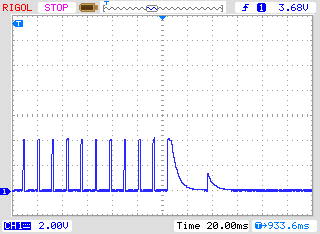
\includegraphics[]{../PNG/IRFU120gate.png}
\caption{Messung der Schwellspannung eines N-Kanal-MOSFET}
\label{fig:eleven}
\end{figure}

\subsection{Messung von Dioden}
\label{sec:diode}
Wenn Strom bei den Vortests festgestellt wurde, wird das Bauteil auf Diodenverhalten gepr\"uft.
Die Flu"sspannung mit dem \(680\Omega\) Widerstand mu"s zwischen 0,15V und 4,64V liegen.
Die Flu"sspannung mit dem \(680\Omega\) Widerstand mu"s gr\"o"ser als 1,125 Mal der Flu"sspannung mit dem
 \(470k\Omega\) Widerstand sein und acht Mal die Flu"sspannung mit dem \(470k\Omega\) Widerstand mu"s
gr\"o"ser als die Flu"sspannung mit dem \(680\Omega\) Widerstand sein.
Ich hoffe, da"s dieses Verhalten immer eine Diode ist.

\subsection{Ergebnisse der verschiedenen Messungen}
Die folgenden drei Tabelle zeigen die Ergebnisse verschiedener Bauteile mit
verschiedenen Software Konfigurationen von ATmega8 und ATmega168 Prozessoren.

\begin{table}[H]
  \begin{center}
    \begin{tabular}{| l | c | c | c |}
    \hline
     Diode & Mega8@8MHz & Mega168 @8MHz & Mega168 @8MHz \\
     Type  & Signatur 1E9307 & Signatur 1E9406 & Signatur 1E9406 \\
           & WITH\_AUTO\_REF &  & WITH\_AUTO\_REF \\
           &                 &  & AUTOSCALE\_ADC \\
    \hline
    \hline
1N4148 & Diode, 721mV, 0pF & Diode, 729mV, 0pF & Diode, 725mV, 0pF\\
    \hline
1N4150 & Diode, 678mV, 0pF & Diode, 681mV, 0pF & Diode, 682mV, 0pF\\
    \hline
BA157 & Diode,623mV, 17pF & Diode, 631mV, 16pF & Diode, 620mV, 15pF\\
    \hline
BY398 & Diode, 541mV, 0pF & Diode, 553mV, 0pF & Diode, 542mV, 0pF\\
    \hline
1N4007 & Diode, 654mV, 13pF & Diode, 665mV, 9pF & Diode, 658mV, 11pF\\
    \hline
LED green & Diode, 1954mV, 6pF & Diode, 1970mV, 6pF & Diode, 1951mV, 4pF\\
    \hline
ZPD2,7 & 2xDi, 729mV, 2659mV & 2xDi, 738mV, 2674mV & 2xDi, 730mV, 2656mV \\
    \hline
BU508A B+E & Diode, 613mV, 5201pF & Diode, 621mV, 5285pF & Diode, 611mV, 5344pF\\
    \hline
BU508A B+C & Diode, 595mV, 261pF & Diode, 597mV, 267pF & Diode, 591mV, 272pF\\
    \hline
    \end{tabular}
  \end{center}
  \caption{Me"sergebnisse der Dioden-Tests}
  \label{tab:diodes} 
\end{table}

\begin{table}[H]
  \begin{center}
    \begin{tabular}{| l | c | c | c |}
    \hline
     Transistor & Mega8@8MHz & Mega168 @8MHz & Mega168 @8MHz \\
     Type   & Signatur 1E9307 & Signatur 1E9406 & Signatur 1E9406 \\
           & WITH\_AUTO\_REF &  & WITH\_AUTO\_REF \\
           &                 &  & AUTOSCALE\_ADC \\
    \hline
    \hline
BU508A & NPN, B=9, 613mV & NPN, B=9, 621mV & NPN, B=9, 615mV\\
    \hline
2N3055 & NPN, B=21, 617mV & NPN, B=21, 626mV & NPN, B=21, 625mV\\
    \hline
BC546B & NPN, B=381, 780mV & NPN, B=376, 777mV & NPN, B=387, 771mV\\
    \hline
BC556B & PNP, B=266, 790mV & PNP, B=429, 787mV & PNP, B=266, 790mV\\
    \hline
BC639 & NPN, B=180, 722mV & NPN, B=180, 733mV & NPN, B=188, 724mV\\

    \hline
BC640 & PNP, B=185, 716mV & PNP, B=227, 725mV & PNP, B=187, 719mV\\
    \hline
AC128 (Ge.) & PNP, B=68, 270mV & PNP, B=64, 269mV & PNP, B=66, 271mV\\
    \hline
BC517 & NPN, B=26996, 1419mV & NPN, B=28220, 1413mV & NPN, B=28250, 1404mV\\
    \hline
BC516 & PNP, B=65535, 1430mV & PNP, B=65535, 1420mV & PNP, B=65535, 1417mV\\
    \hline
BRY55/200 & Thyristor & Thyristor & Thyristor\\
    \hline
    \end{tabular}
  \end{center}
  \caption{Me"sergebnisse der Tests mit bipolaren Transistoren}
  \label{tab:bipolar} 
\end{table}

\begin{table}[H]
  \begin{center}
    \begin{tabular}{| l | c | c | c |}
    \hline
     FET & Mega8@8MHz & Mega168 @8MHz & Mega168 @8MHz \\
    Type    & Signatur 1E9307 & Signatur 1E9406 & Signatur 1E9406 \\
           & WITH\_AUTO\_REF &  & WITH\_AUTO\_REF \\
           &                 &  & AUTOSCALE\_ADC \\
    \hline
    \hline
BS170 & N-E-MOS,D, 2616mV & N-E-MOS,D, 2562mV & N-E-MOS,D, 2564mV \\
      &  66pF             &  67pF  &  68pF \\
    \hline
J310 & N-JFET & N-JFET & N-JFET\\
    \hline
IRFU120N & N-E-MOS,D, 4151mV & N-E-MOS,D, 4156mV & N-E-MOS,D, 4153mV\\
     & 922pF  & 894pF  & 933pF \\
    \hline
IRFU9024 & P-E-MOS,D, 3525mV & P-E-MOS,D, 3525mV & P-E-MOS,D, 3534mV\\
     & 960pF & 926pF & 965pF \\
    \hline
ZVP2106A & P-E-MOS,D, 3217mV & P-E-MOS,D, 3220mV & P-E-MOS,D, 3217mV\\
  & 115pF & 114pF & 113pF \\
    \hline
ZVNL120A & N-E-MOS,D, 1560mV & N-E-MOS,D, 1535mV & N-E-MOS,D, 1535mV \\
  & 140pF & 138pF  & 138pF \\
    \hline
    \end{tabular}
  \end{center}
  \caption{Me"sergebnisse der MOS Transistor Tests}
  \label{tab:mos} 
\end{table}
